%% -*- coding:utf-8 -*- 
\begin{figure}
\centering

\ifpdf
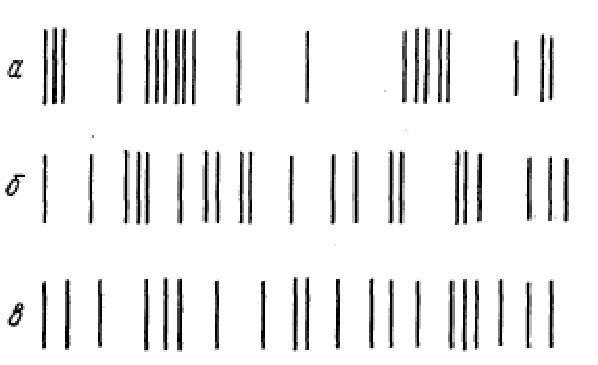
\includegraphics[angle=0, width=0.5\textwidth]
{./part3/nonclass/nonclassphoto.pdf}
\else
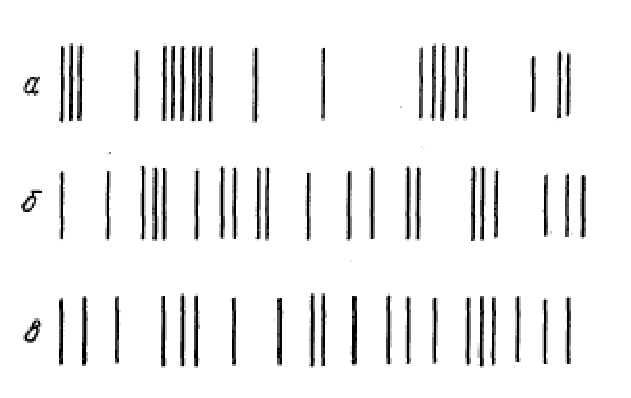
\includegraphics[angle=0, width=0.5\textwidth]
{./part3/nonclass/nonclassphoto.eps}
\fi
%\input ./part3/nonclass/picnonclass1.tex

\caption{Примеры реализаций фотоотсчетов, соответствующие различным
  статистическим свойствам света: а) группировка и свехпуассоновская
  статистика, б) пуассоновская статистика, в) антигруппировка и
  субпуассоновская статистика (по данным работы \cite{bNonclassSmirnovTroshin}). }
\label{figPart3Nonclass1}
\end{figure}
